\chapter{Martas Work}

\section{BLOB-Analysis}
A common problem when dealing with images is to determine if the image data contains a particular object or shape. The term BLOB stands for Binary Large Objects and refers to a region of connected pixels in a binary image. This technique is used to extract meaningful information from images, separate the pixels by detecting the points or regions that differ in properties like brightness or color changes (i.e., their value), and classify them into two categories: the foreground (pixels with a non-zero value) and the background (pixels with a zero value).
Therefore, BLOB analysis will be split in three main steps: \textit{Extraction} of the BLOBs, \textit{representation} of the BLOBs and lastly, \textit{classification} of the BLOBs to know which ones belong to the expected type.
\subsection{BLOB Extraction}
To isolate BLOBs in a binary image, we need to define first if two pixels are connected or not. This is done by applying algorithms that will help to determine the connectivity of the pixels, but also the number of BLOBs contained in an image. The most common used connectivities in BLOB extraction are the 8-connectivity and the 4-connectivity kernels. Whereas the 8-connectivity kernel is more accurate, it also requires more computations and consequently, needs more time to process the image.

%% add picture here

\subsubsection{Grass-Fire Algorithm}
One of these connected component labeling algorithm is the \textbf{Recursive Grass-Fire Algorithm}, used to erode images but also to track the pixels locations to create a region.
To explain this algorithm, we will use both 8-connectivity and 4-connectivity kernels to illustrate how these choices can affect to the final result.

\begin{figure}[htbp]
\centering
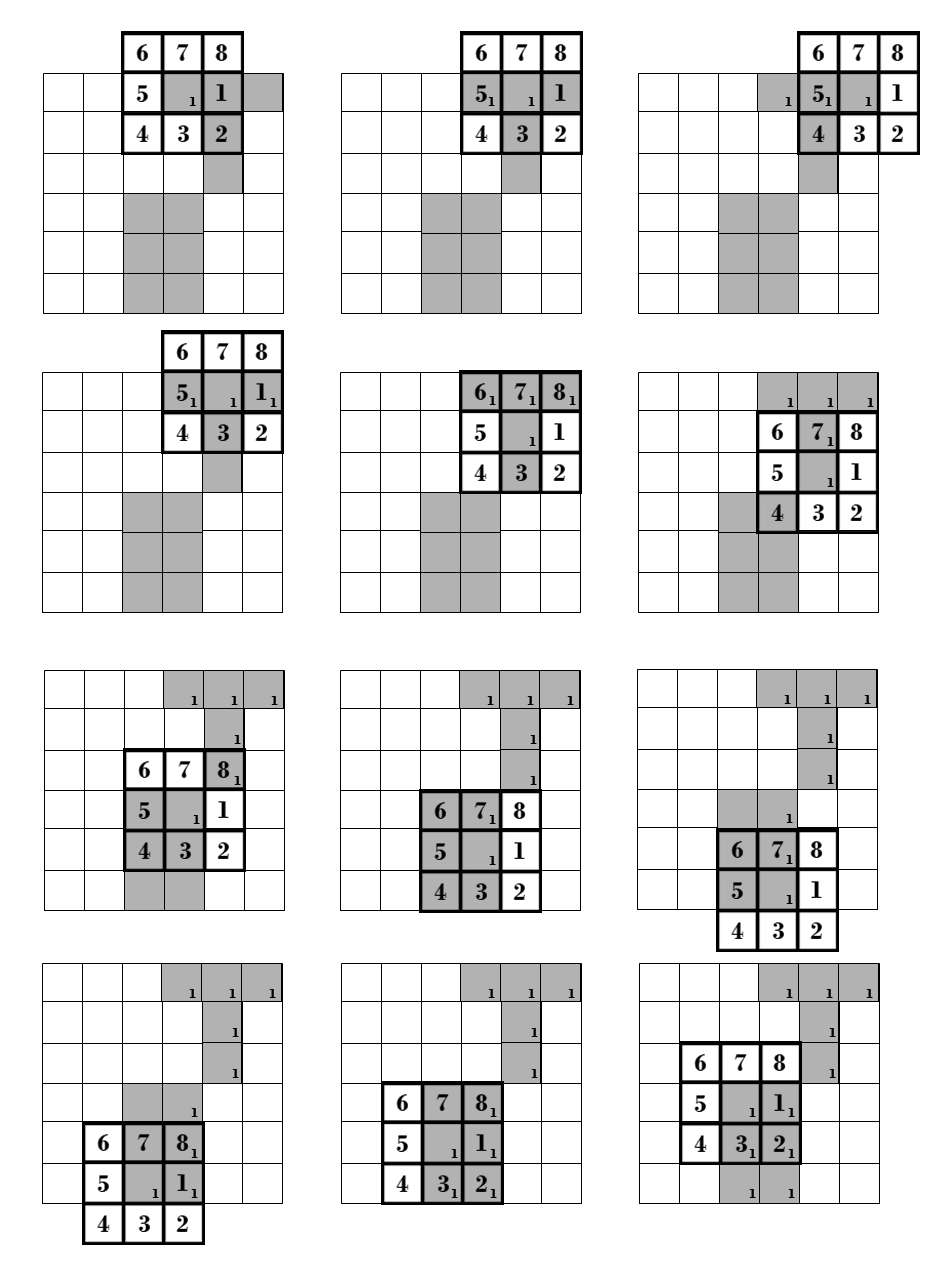
\includegraphics[width=0.8\textwidth]{Pictures/Theory/8connec_kernel.png}
\caption{8 connectivity labeling kernel detects 1 single object}
\label{fig:8connecK}
\end{figure}

As we can see on figure \eqref{fig:8connecK}, the Grass-Fire algorithm scans the whole image from the upper-left side to the right bottom, row by row. When the kernel finds a non-zero pixel value it centers its attention on it and burns it. Then the algorithm looks in the possible directions around that pixel to check if one of those pixels is connected to the previous one, and therefore, is an object. The way the algorithm will do this will depend on the connectivity used (for a 8-connectivity kernel, the algorithm will look into 8 directions, but for the 4-connectivity kernel, the algorithm will look in 4 directions).
Whenever it finds an object, the algorithm labels the pixel on the output image and then burns that pixel on the input image in order to turn it into a zero and ensure that the pixel will not be part of a new grassfire.
The algorithm looks now on the possible directions around that pixel, starting with the pixel on the right (see kernel picture \eqref{fig:8connecK}). Once it finds a non-zero pixel value, the algorithm centers its attention on it and restarts the process again labeling the pixel with the number of the previous one. At the end of that row the algorithm will check the surrounding pixels on the row below. If a non-zero pixel value is found, the algorithm will continue the process of burning and labeling pixels, otherwise the algorithm will starts its way back to the beginning checking one by one surrounding pixels to verify that it has checked all the possible directions and non-zero pixels values.
Comparing the figure \eqref{fig:8connecK} and the figure \eqref{fig:4connecK}, we can realize how the choice of a certain connectivity kernel will affect the final result of the algorithm using a same picture. Although the 8-connectivity kernel is more accurate it seems to be unable to separate the different objects correctly, whereas the 4-connectivity kernel finds the different objects performing less operations.

\begin{figure}[htbp]
\centering
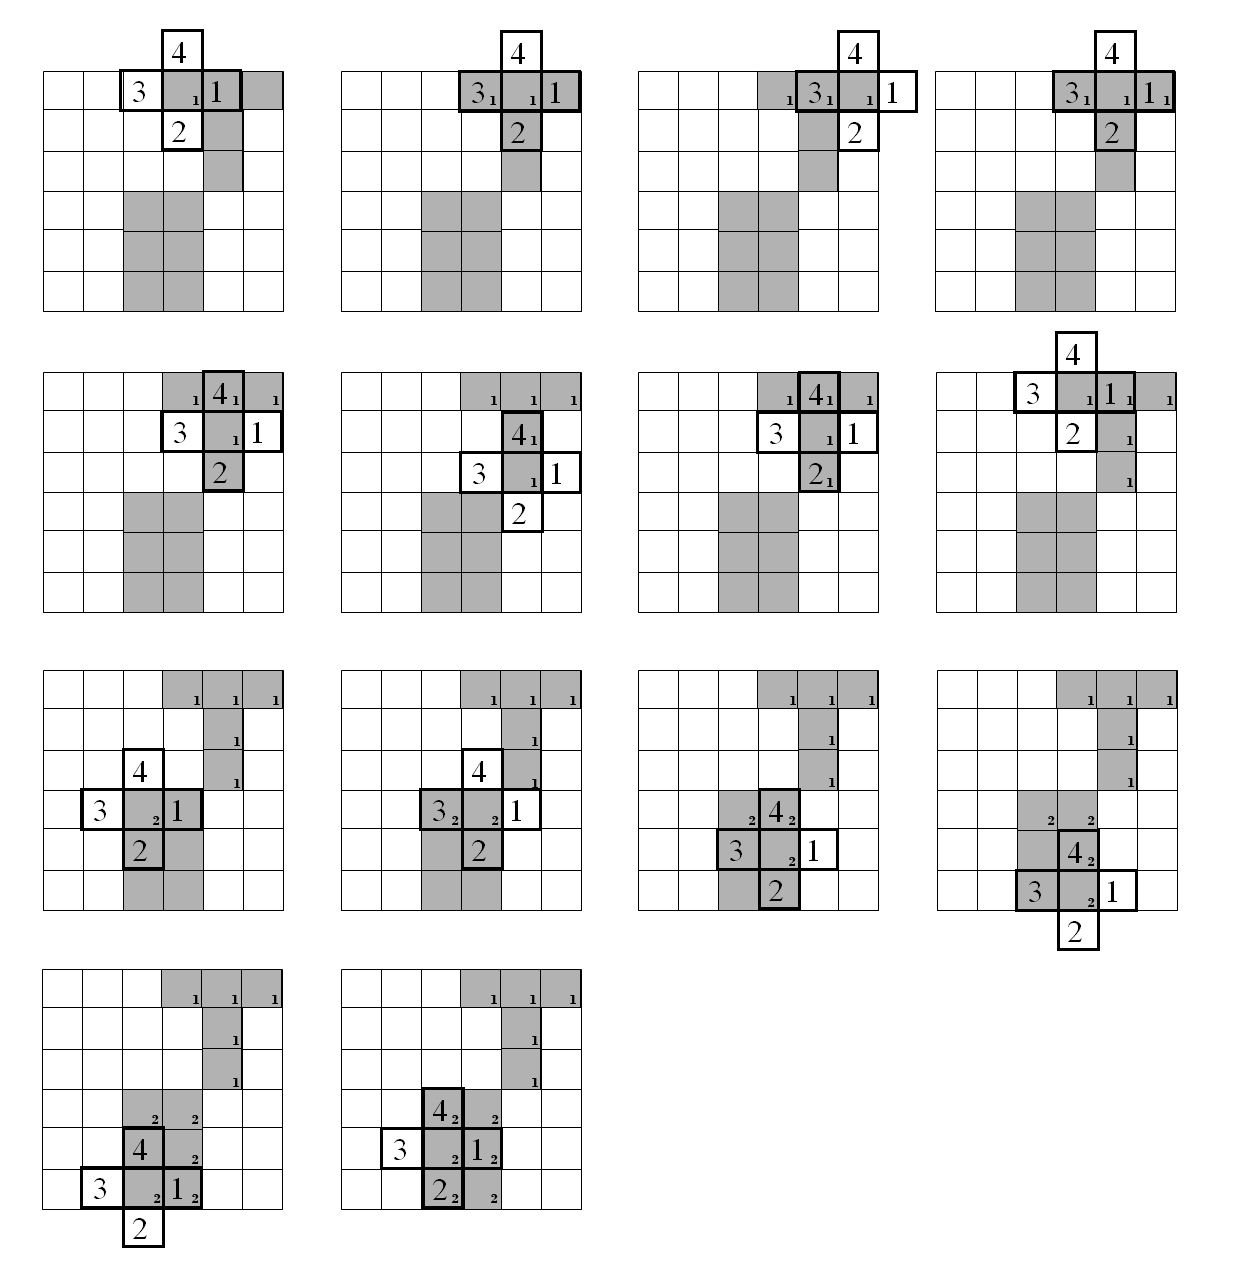
\includegraphics[width=0.75\textwidth]{Pictures/Theory/4connec_kernel.png}
\caption{4 connectivity labeling kernel detects 2 objects}
\label{fig:4connecK}
\end{figure}



Figure \eqref{fig:4connecK}

\subsection{BLOB Representation}
The classification of the BLOBs is made by creating a \textit{prototype model} of the object that we are looking for, in order to state the features that it should accomplish, and the deviations that would be acceptable. This process consist of two steps: determining the features of the BLOB and matching the features with the objects found to determine if they are part of the type that we were looking for.

Hence a few features like the \textbf{area}, the \textbf{perimeter} and the \textbf{circularity} will be calculated.
\subsubsection{The features}

\begin{itemize}
\item Area

The importance of calculating features like the \textbf{area} of a BLOB is well understood if we keep in mind that one of the first steps while classifying the detected objects is to delete those that are bigger or smaller than the expected ones. One way of doing this is by calculating the area of the BLOBs.

\item Bounding box and Bounding circle

Both \textbf{bounding box} and \textbf{bounding circle} are features that operate in a similar way, as the particularity of these features is to enclose those objects that fit into a specific box or circle. The difference between these two besides the shape, is the way it operates. While the \textbf{bounding box} is the minimum rectangle and it checks the four pixels with the minimum and maximum x and y values, the \textbf{bounding circle} is the minimum circle and needs to find first the center of the BLOB.

\item Convex hull

It's the minimum convex polygon which contains the BLOB. Starting from the topmost pixel of the BLOB and searching on the right along a horizontal line and in the clockwise angle till, it finds a BLOB pixel and creates the first side of the polygon.

\item Bounding box ratio
This is the height of the bounding box divided by the width, indicating in this way the lengthening of the BLOB.
\item Compactness
The compactness of a BLOB is the ratio of the BLOB's area to the ratio of the bounding box.

\begin{equation}
	\begin{aligned}
	\text{Compactness}=\displaystyle\frac{BLOB's Area}{width\cdot{height}}
	\label{Compact}
	\end{aligned}
\end{equation}


\item Center of mass
In physics, the center of mass is the unique point where the weighted relative position of the distributed mass sums to zero. The common example to explain this would be the place where you have to place your finger on an object in order to have it balanced.

The distribution of mass is balanced around the center of mass and the average of the weighted position coordinates of the distributed mass defines its coordinates. On a binary image, this center will be the average x and y positions of the object on the image.

Its coordinates can be found using the formula:

\begin{equation}
	\begin{aligned}
  		\ \text{Center of Mass} = \left\{ \begin{array}{ll}
         x_{c}=\displaystyle\frac{1}{N} \displaystyle\sum_{i=1}^N x_{i}\\
         y_{c}=\displaystyle\frac{1}{N} \displaystyle\sum_{i=1}^N y_{i}
        \end{array} \right . \ 
 	\end{aligned}
\end{equation} 


Where N is the number of pixels in the BLOB and x i and y i are the coordinates of each single pixel inside that BLOB. In some situation where we will need to calculate the center of mass of an object with annexed parts, a median or an erosion before using the previous formula.
\item Center of the bounding box
As the bounding box is a rectangle that surrounds the BLOB, the center of the bounding box is an approximation of the center of mass and can be found with the formula:

\begin{equation}
	\begin{aligned}	x_{bb}=x_{min}+\displaystyle\frac{x_{max}-x_{min}}{2}=x_{min}+\displaystyle\frac{x_{max}}{2}-\displaystyle\frac{x_{min}}{2}=\displaystyle\frac{x_{min}+x_{max}}{2}
	\label{BoundingBoxCenterX}
	\end{aligned}
\end{equation}

\begin{equation}	
	\begin{aligned}
	y_{bb}=y_{min}+\displaystyle\frac{y_{max}-y_{min}}{2}=y_{min}+\displaystyle\frac{y_{max}}{2}-\displaystyle\frac{y_{min}}{2}=\displaystyle\frac{y_{min}+y_{max}}{2}
	\label{BoundingBoxCenterY}
	\end{aligned}
\end{equation}


\item Perimeter

Scanning along the border of the BLOB and summing the pixels we obtain the length of the contour of the BLOB. In Image Processing, this could be done by using morphology techniques like erosion to get a smaller version of the object and then subtracting this to the input image in order to get the edges.

\item Circularity

Circularity is a very common shape factor that depends on the \textbf{Perimeter} and the \textbf{Area}. There are several ways to define how circular an object can be, but usually we apply the ratio to get a value lower or equal to 1 that will indicate how circular the BLOB is.

\begin{equation}	
	\begin{aligned}
	{Circularity}=\displaystyle\frac{BLOB's \;\; Perimeter}{2 \; \sqrt{\mathstrut \: \Pi \: \cdot \: {BLOB's \;\; Area}}}
	\label{Circularity}
	\end{aligned}
\end{equation}

After all the feature's extractions, a binary object can be defined by its features value that would be stored into a \textit{feature vector} in order to have a list where to start our BLOB's classification.

\end{itemize}


% IMAGE WITH OBJECTS AND TABLE WITH DATA

\subsection{BLOB Classification}

Once we have extracted and represented each object on the binary image by its features, we need to determine the minimum characteristics that the object have to accomplish so that it can be selected.
For this reason, we will define a \textit{prototype model} based on ideal measurements that is used as a reference to which the extracted values are compared. As the real object will not be perfect, a deviation is needed to create a tolerance range.
Using two features like the circularity and the area we will create a frame, also known as a \textit{box classifier}, and every object belonging to that \textit{feature space}, also know as \textit{decision region}, will then be understood as a desired object.

Another way to achieve this would be to create a \textit{statistical classifier} using means and variances of the features, where the task would be to measure the distance between a new feature vector and the prototype. The smaller the distance between those two is, the more likely the object will be part of the same type. But before getting to this point, we need to threshold the distance and consequently have a binary decision region like the \textit{box classifier}.
This time, the region will not be a rectangle but an ellipse, and is commonly known as the \textit{weighted Euclidean distance}.

\begin{equation}	
	\begin{aligned}
{WED(\vec{f}_{i} \; , \: prototype)} \: = \: \sqrt{\mathstrut \:  \displaystyle\frac{(f_{i}(cir) \: - \: mean(cir))^2}{variance(cir)} \: + \: \displaystyle\frac{(f_{i}(area) \: - \: mean(area))^2}{variance(area)}}
\label{Euclidean}
	\end{aligned}
\end{equation}

The final result is the distance between the vector {$\vec{f}_{i}$} and the prototype. The values of {$f_{i}(cir)$} and {$f_{i}(area)$} correspond to the circularity and the area of every object found on the binary image. For an image with a number of N different features, the result would be obtained by summing:


\begin{equation}	
	\begin{aligned}
{WED(\vec{f}_{i} \; , \: prototype)} \: = \: \displaystyle\sum_{i=1}^N \: \: \sqrt{\mathstrut \:  \displaystyle\frac{(f_{i}(m_{j}) \: - \: mean(m_{j}))^2}{variance(m_{j})}}
\label{Euclidean1}
	\end{aligned}
\end{equation}

Where {$m_{j}$} is the {$jth$} feature. When the variances of the features are the same all along the list of values, we can ignore it and calculate the Euclidean distance (ED), where the region is a circle in 2D.

\begin{equation}	
	\begin{aligned}
{ED(\vec{f}_{i} \; , \: prototype)} \: = \: \displaystyle\sum_{i=1}^N \: \sqrt{\mathstrut (f_{i}(m{j}) - mean(m_{j}))^2}
\label{Euclidean2}
	\end{aligned}
\end{equation}

But before we can calculate the distances, we need to normalize the values to the same scale and interval.

Therefore, the Area would be done by:

\begin{equation}	
	\begin{aligned}
{Area \: feature} \: = \: min \begin{Bmatrix} \displaystyle\frac{Area\:of\:BLOB}{Area\:of\:Model}, & \displaystyle\frac{Area\:of\:Model}{Area\:of\:BLOB}\end{Bmatrix}
\label{NormArea}
	\end{aligned}
\end{equation}

The Circularity can also be normalized in the same:

\begin{equation}	
	\begin{aligned}
{Circularity \: feature} \: = \: min \begin{Bmatrix} {Circularity}, & \displaystyle\frac{1}{Circularity}\end{Bmatrix}
\label{NormCirc}
	\end{aligned}
\end{equation}